
El siguiente instrumento fue diseñado con el propósito de validar la relevancia
de la aplicación propuesta en el contexto del consumo de dispositivos
electrónicos.

\textit{El instrumento será aplicado en formato digital. Las preguntas cerradas 
cuentan con opciones de respuesta predefinidas según su tipo (dicotómicas, 
opción múltiple o respuesta abierta).}

\bigskip

\noindent Esta es una encuesta enfocada en conocer la forma en la que tomas
decisiones al momento de comprar teléfonos inteligentes (smartphones) y laptops,
desde lo que tomas en cuenta para elegir el producto, hasta que te hace querer
comprarlo.

\noindent  La presente encuesta se realiza con el fin de recopilar datos reales
para nuestra investigación de la materia ``Taller de Investigación I'' titulada:
``Obsolescencia Programada: Cómo Erradicarla a Través de la Honestidad y
Veracidad de la Información en Smartphones y Laptops mediante los Principios de
la Economía Circular''. Debido a la naturaleza de la investigación te pedimos
que seas lo más honesto posible ya que de esa forma podremos hacer que la
investigación se fundamente y logre un objetivo real.

\noindent La información aquí presentada es para fines documentales y todo se
presentará de forma anónima manteniendo tus datos personales en privado,
respetando tu privacidad.

% ─── BLOQUE 1: Conocimiento conceptual ───────────────────────────────────────
\subsection*{Sección 1: Conocimiento sobre términos clave}

\begin{enumerate}
    \item ¿Has escuchado el término \textit{obsolescencia programada}? \\
    \textbf{Sí} \quad \textbf{No}
    
    \item En caso afirmativo, ¿sabes o tienes una idea de lo que significa?\\
    \textbf{Sí} \quad \textbf{No}

    \item ¿Has escuchado el término \textit{economía circular}? \\
    \textbf{Sí} \quad \textbf{No}

    \item En caso afirmativo, ¿sabes o tienes una idea de lo que significa? \\
    \textbf{Sí} \quad \textbf{No}
    
    \item ¿Has escuchado sobre el término \textit{derecho a reparar}? \\
    \textbf{Sí} \quad \textbf{No}
    
    \item En caso afirmativo, ¿sabes o tienes una idea de lo que significa? \\
    \textbf{Sí} \quad \textbf{No}
    
    \item ¿Has escuchado el término \textit{greenwashing} (green: verde –
    washing: lavado)? \\
    \textbf{Sí} \quad \textbf{No}
    
    \item En caso afirmativo, ¿sabes o tienes una idea de lo que significa? \\
    \textbf{Sí} \quad \textbf{No}
\end{enumerate}

% ─── BLOQUE 2: Comportamiento de compra ──────────────────────────────────────
\subsection*{Sección 2: Comportamiento de compra}

\begin{enumerate}[resume]
    \item ¿Has comprado alguna vez un teléfono inteligente? \\
    \textbf{Sí} \quad \textbf{No}

    \item En caso afirmativo, ¿cuándo fue la última vez que compraste un
    teléfono inteligente? \\
    \textbf{Sí} \quad \textbf{No}

    \item ¿Cuál fue la razón por la que decidiste comprarlo? Ejemplo: la
    reparación era más costosa que adquirir uno nuevo; las actualizaciones ya no
    eran compatibles con el dispositivo; resultaba más conveniente
    económicamente reemplazarlo, entre otras razones. \\
    \underline{\hspace{\linewidth}} \\
    \underline{\hspace{\linewidth}}

    \item ¿Has comprado alguna vez una laptop? \\
    \textbf{Sí} \quad \textbf{No}

    \item En caso afirmativo, ¿cuándo fue la última vez que compraste una
    laptop? \\
    \textbf{Sí} \quad \textbf{No}

    \item ¿Cuál fue la razón por la que decidiste comprarla? \\
    \underline{\hspace{\linewidth}} \\
    \underline{\hspace{\linewidth}}

\end{enumerate}

% ─── BLOQUE 3: Toma de decisiones ────────────────────────────────────────────
\subsection*{Sección 3: Toma de decisiones}

\begin{enumerate}[resume]

    \item En el momento en que decides comprar un producto en general.
    ¿Por qué razón consideras que tomaste la decisión de comprarlo? \\
    \underline{\hspace{\linewidth}} \\
    \underline{\hspace{\linewidth}}

    \item ¿Alguna vez has comprado algo que después te parece una compra
    innecesaria? \\
    \textbf{Sí} \quad \textbf{No}

    \item En caso afirmativo, ¿consideras que esto sucede por la publicidad que
    te hace creer que es algo necesario en tu vida? \\
    \textbf{Sí} \quad \textbf{No}

    \item Imagina que ves anuncios publicitarios de algo que te interesa
    comprar. ¿Qué es lo que pasa por tu mente al verlos? \\
    \underline{\hspace{\linewidth}} \\
    \underline{\hspace{\linewidth}}

    \item Recuerda anuncios que has visto sobre productos que no tenías en tu
    lista de compras y que terminaste comprando. ¿Qué te hizo comprarlos? \\
    \underline{\hspace{\linewidth}} \\
    \underline{\hspace{\linewidth}}

\end{enumerate}

% ─── BLOQUE 4: Estímulos visuales ────────────────────────────────────────────
\subsection*{Sección 4: Reacción ante estímulos publicitarios}

\begin{enumerate}[resume]

    \item A continuación se presenta un anuncio publicitario de un dispositivo
    electrónico. Obsérvalo con atención.

    \begin{center}
        \fbox{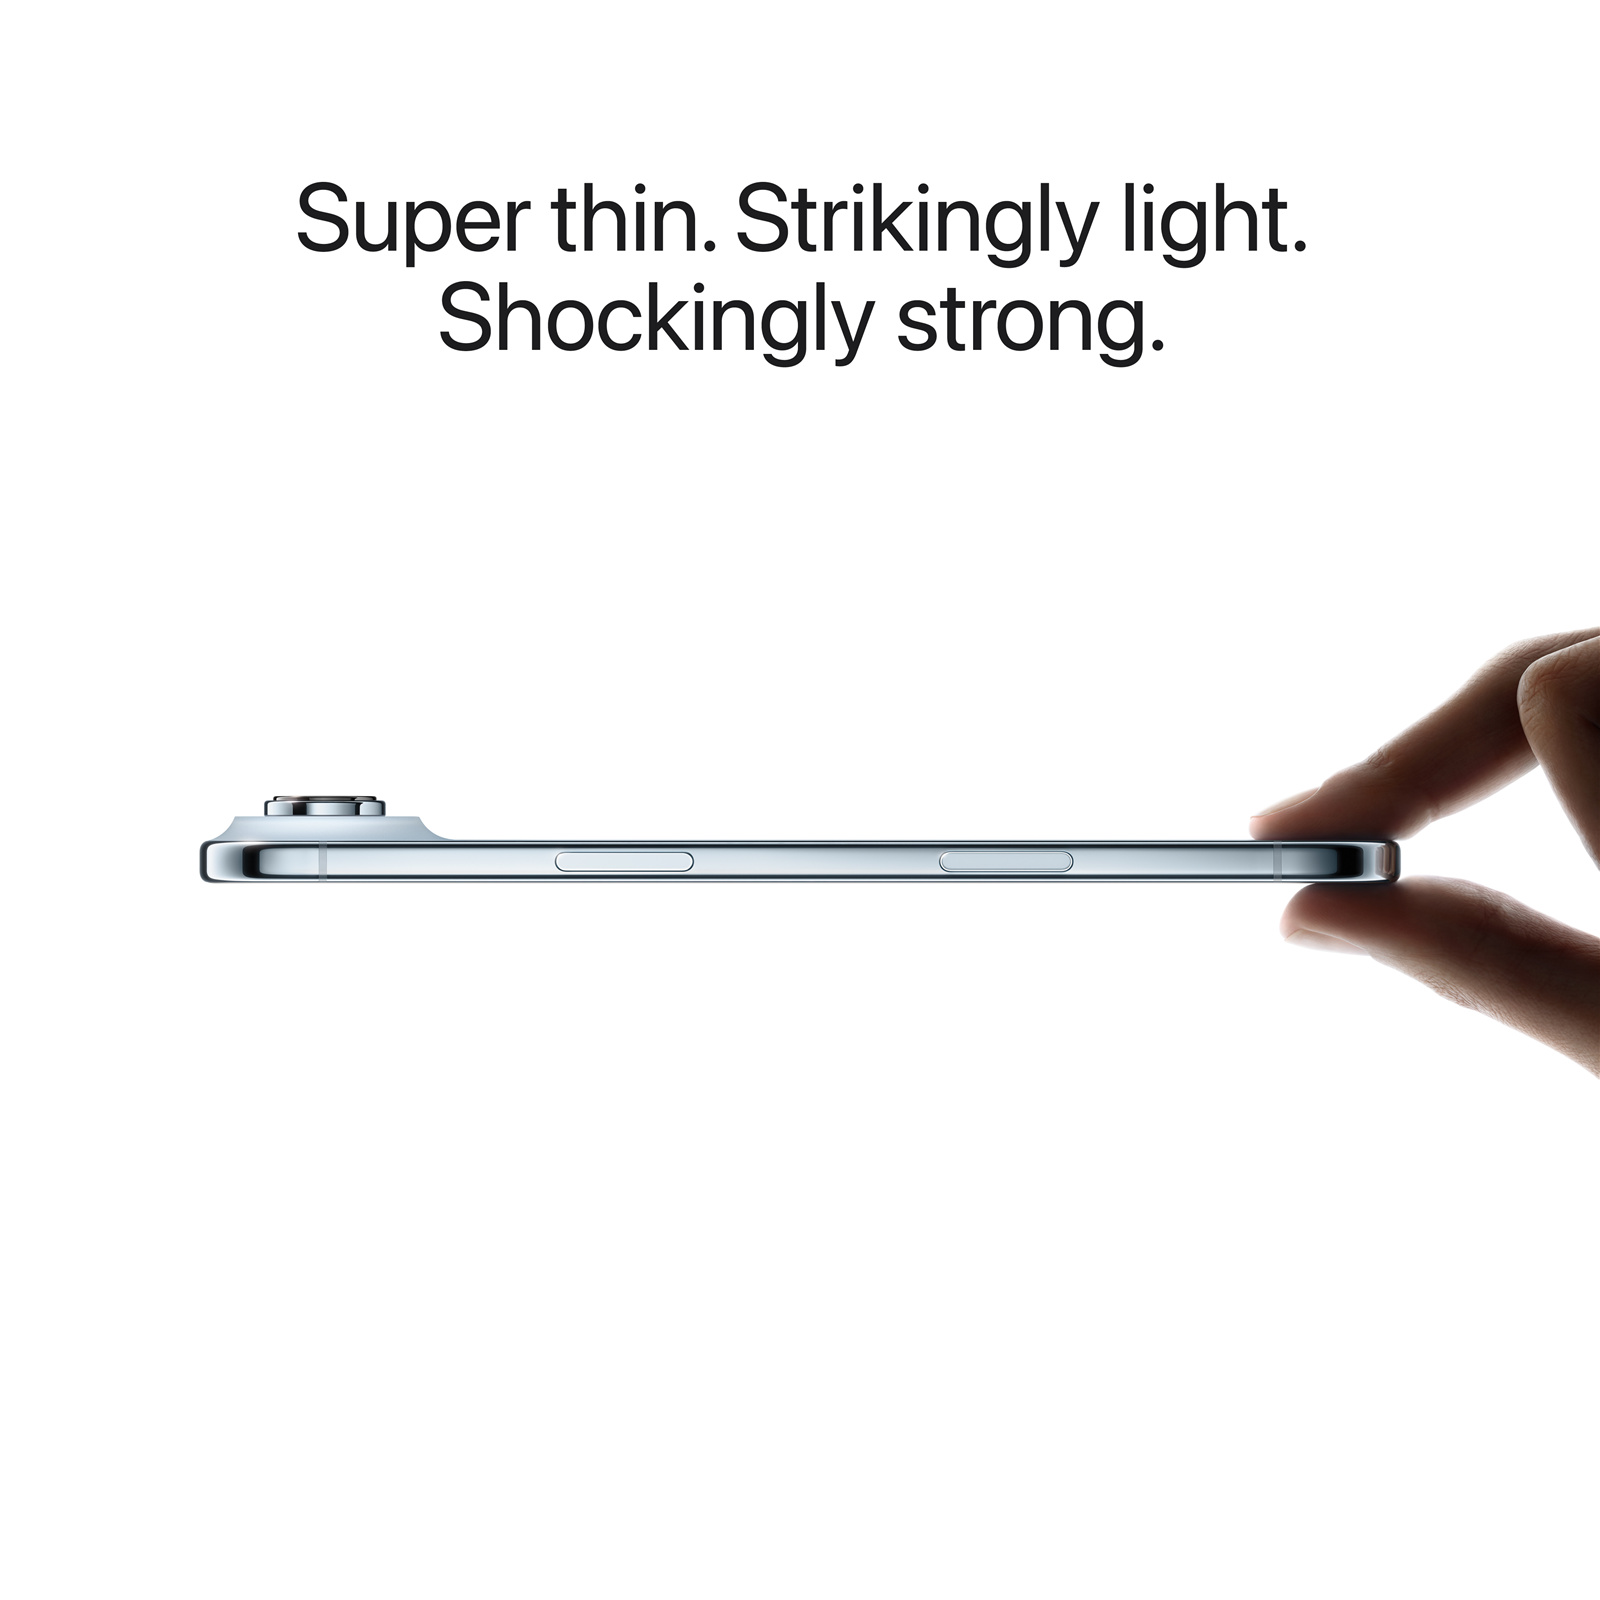
\includegraphics[width=0.5\textwidth]{imagenes/anuncio01.png}}
    \end{center}

    ¿Qué piensas después de ver este anuncio? \\
    \underline{\hspace{\linewidth}} \\
    \underline{\hspace{\linewidth}}

    \item A continuación se presenta un segundo anuncio.

    \begin{center}
        \fbox{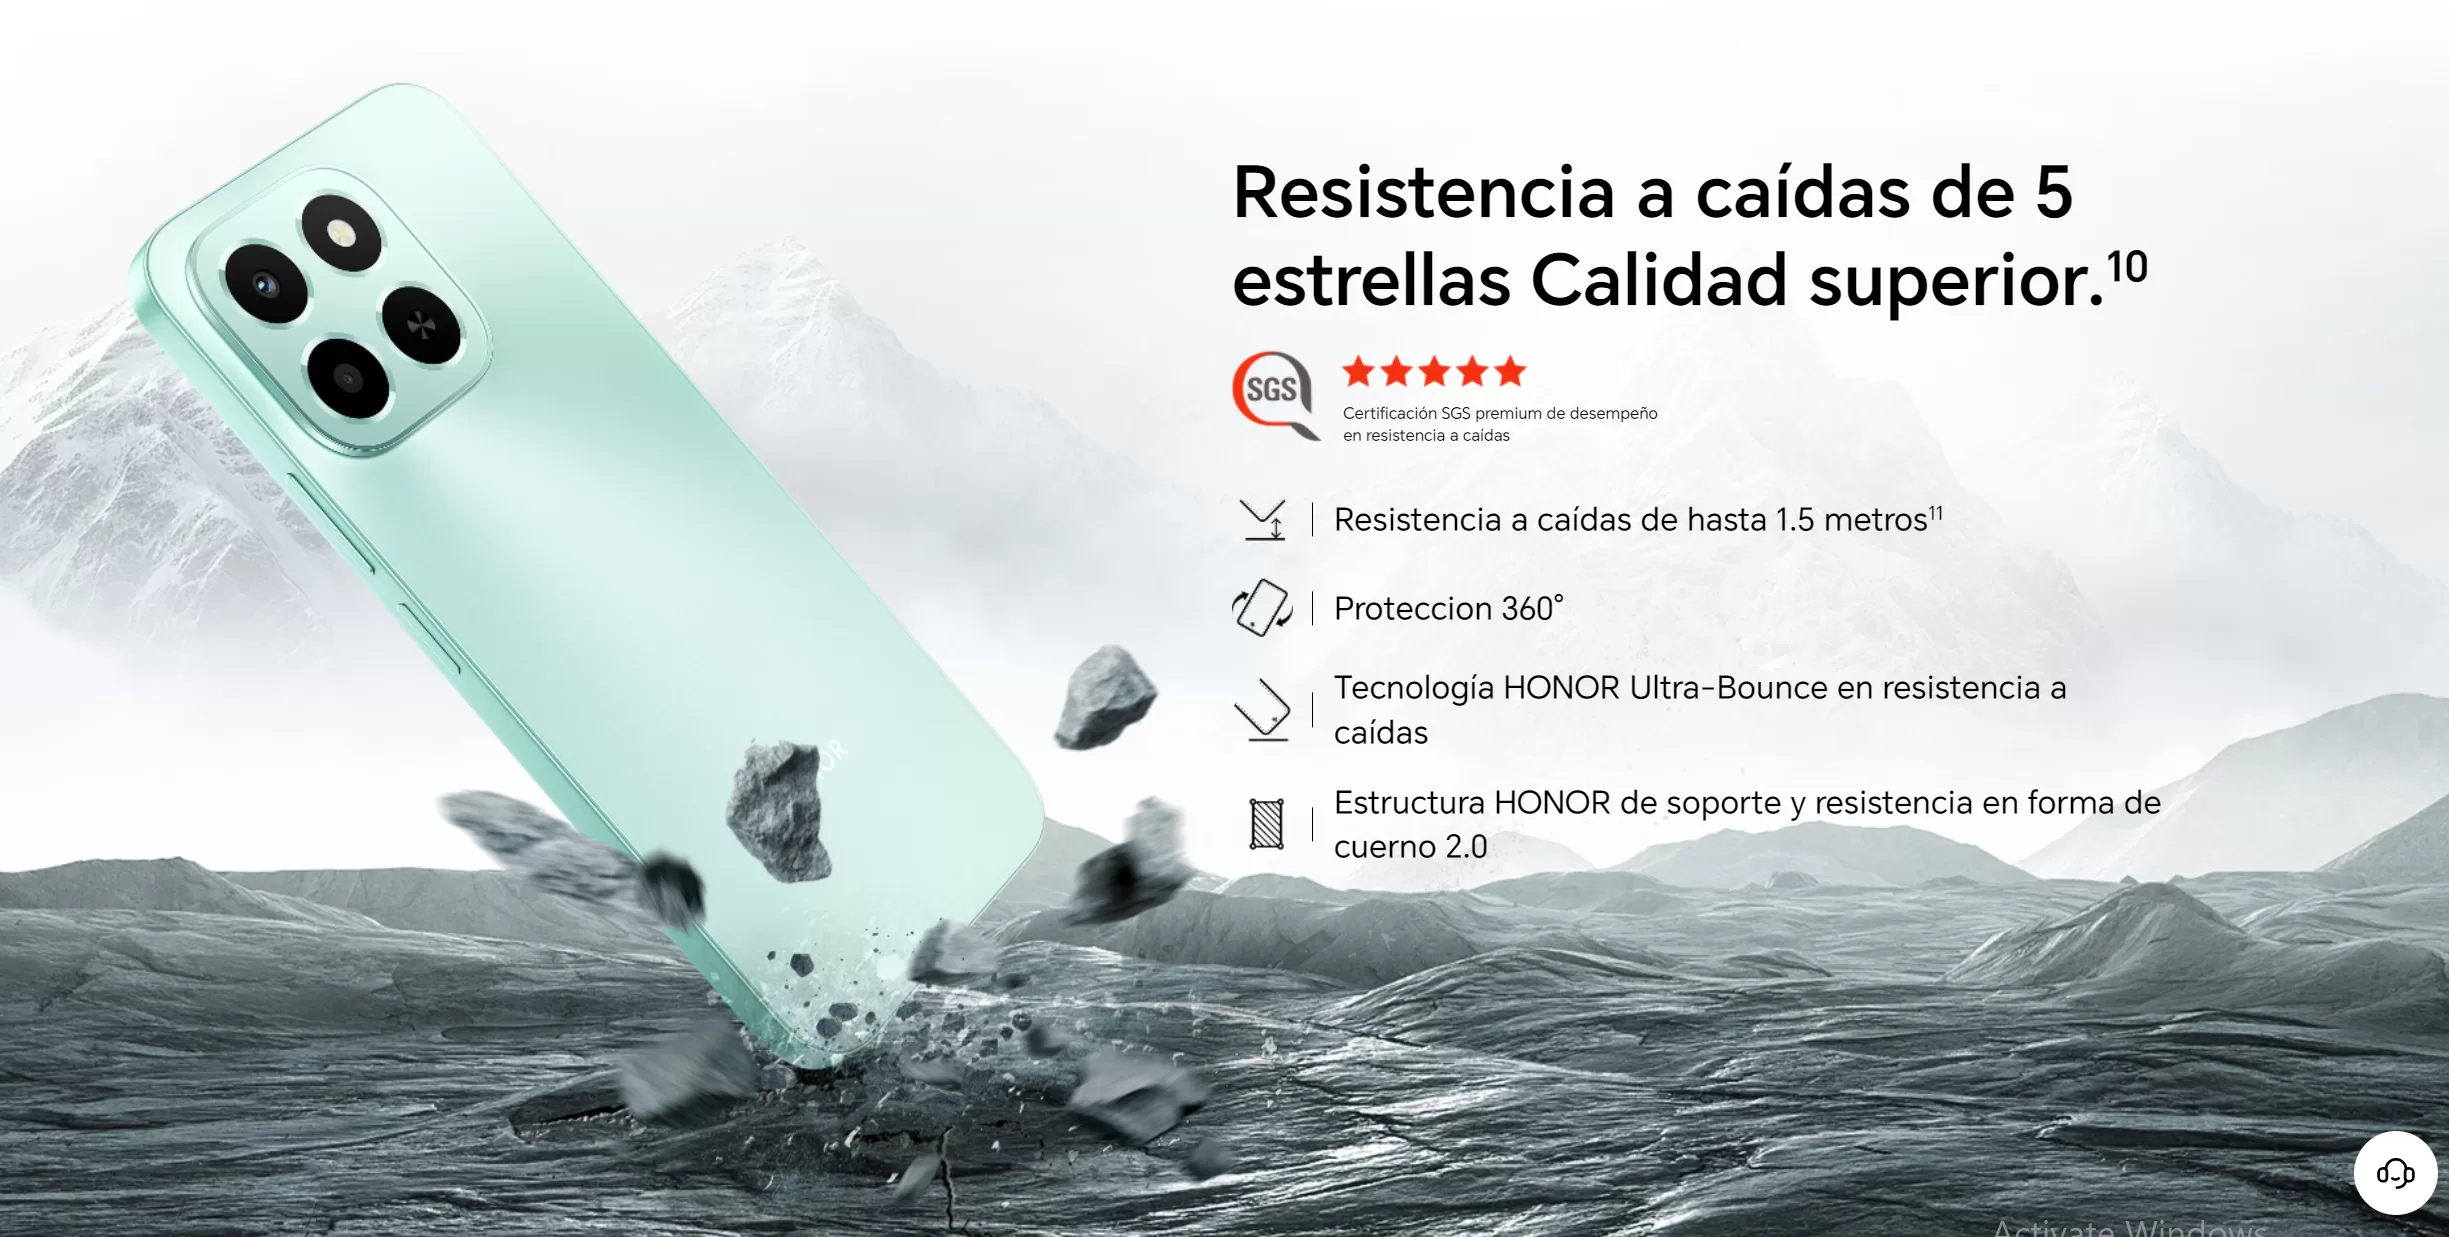
\includegraphics[width=0.8\textwidth]{imagenes/anuncio02.png}}
    \end{center}

    ¿Qué piensas o qué sensación te deja después de ver este anuncio? \\
    \underline{\hspace{\linewidth}} \\
    \underline{\hspace{\linewidth}}

\end{enumerate}

% ─── BLOQUE 5: Durabilidad y reparación ──────────────────────────────────────
\subsection*{Sección 5: Durabilidad, reparación y ciclo de vida}

\begin{enumerate}[resume]

    \item ¿Alguna vez te has preguntado por qué, después de aproximadamente 3 o
    4 años, sueles cambiar tus dispositivos electrónicos? \\
    \textbf{Sí} \quad \textbf{No}

    \item Pensando en el año 2011 —hace aproximadamente 15 años— y en cómo era
    el ritmo de vida y la resistencia de los dispositivos en esa época, ¿crees
    que actualmente las cosas están hechas para desecharse? \\
    \textbf{Sí} \quad \textbf{No}

    \item Imagina que tienes la oportunidad de comprar el teléfono que deseas,
    pero debes elegir entre dos opciones respecto a los materiales con los que
    fue fabricado: materiales con los estándares de calidad actuales o
    materiales con los estándares de hace 15 años. ¿Cuál elegirías? \\
    \textbf{Materiales actuales} \quad \textbf{Materiales de hace 15 años}

    \item ¿Cuáles son tus motivos para la respuesta anterior? \\
    \underline{\hspace{\linewidth}} \\
    \underline{\hspace{\linewidth}}

    \item Si tuvieras la opción de reparar tu teléfono inteligente o laptop
    —sabiendo que no quedaría en malas condiciones, que aumentaría su vida útil
    al menos dos años más, que se podría ampliar su memoria, que continuaría
    recibiendo actualizaciones y que el costo sería correspondiente únicamente a
    los materiales y la mano de obra— ¿elegirías repararlo o preferirías comprar
    uno nuevo? \\
    \textbf{Repararlo} \quad \textbf{Comprar uno nuevo}

    \item ¿Cuáles son tus motivos para la respuesta anterior? \\
    \underline{\hspace{\linewidth}} \\
    \underline{\hspace{\linewidth}}

    \item ¿Qué tanto te importa adquirir lo que está de novedad o es lo más
    popular en el mercado? \\
    \textbf{Me importa mucho} \quad \textbf{Me importa un poco} \quad \textbf{No
    me importa}

    \item En caso de que te importe mucho o un poco, ¿cuáles son tus razones
    para querer adquirir productos nuevos cuando los tuyos funcionan
    correctamente? \\
    \underline{\hspace{\linewidth}} \\
    \underline{\hspace{\linewidth}}

\end{enumerate}

% ─── BLOQUE 6: Utilidad de herramienta propuesta ──────────────────────────────────────
\subsection*{Sección 6: Percepción de utilidad de la herramienta propuesta}

\begin{enumerate}[resume]

    \item Cuando vas a comprar un dispositivo electrónico, ¿qué tan difícil 
    te resulta encontrar información clara y confiable sobre el producto?
    
    \textbf{Muy difícil} \quad \textbf{Algo difícil} \quad \textbf{Poco difícil} \quad \textbf{Nada difícil}

    \item Al momento de comprar un dispositivo electrónico, ¿consultas 
    opiniones de otros usuarios antes de tomar tu decisión?
    
    \textbf{Siempre} \quad \textbf{A veces} \quad \textbf{Casi nunca} \quad \textbf{Nunca}

    \item ¿Alguna vez has dejado de comprar un producto porque no encontraste 
    suficiente información confiable sobre él?
    
    \textbf{Sí} \quad \textbf{No}

    \item Imagina una aplicación que, al escanear el código de barras de un 
    dispositivo electrónico, te muestre de forma clara y progresiva: 
    información del fabricante, opiniones de usuarios reales, 
    certificaciones de sostenibilidad y opciones de reparación cercanas 
    a tu ubicación. ¿Qué tan útil considerarías esta herramienta?
    
    \textbf{Muy útil} \quad \textbf{Útil} \quad \textbf{Poco útil} \quad \textbf{Nada útil}

    \item ¿Crees que contar con una herramienta como la descrita anteriormente 
    influiría en tu decisión de compra?
    
    \textbf{Definitivamente sí} \quad \textbf{Probablemente sí} \quad 
    \textbf{Probablemente no} \quad \textbf{Definitivamente no}

    \item ¿Utilizarías una aplicación de este tipo antes de adquirir 
    un dispositivo electrónico?
    
    \textbf{Sí} \quad \textbf{No} \quad \textbf{Tal vez}

\end{enumerate}

\noindent Te agradecemos el tiempo brindado y las respuestas proporcionadas, éstas serán
usadas para poder fundamentar nuestra investigación, si estás interesade en
leerla no dudes en decirnos y cuando haya sido completada te la proporcionamos. 

\noindent Recuerda que para que el mundo cambie debes de cuestionar todo lo que haces y
sobre todo lo que te dicen, nosotros tenemos el poder como consumidores de
cambiar el rumbo. 